%!TEX root = ./template-skripsi.tex
%-------------------------------------------------------------------------------
%                            BAB II
%               KAJIAN TEORI
%-------------------------------------------------------------------------------

\chapter{KAJIAN PUSTAKA}                


\section{Populasi dan Sampel}
Tujuan dari sebuah riset adalah untuk memperoleh informasi dari populasi. Populasi merupakan seluruh kumpulan elemen yang dapat digunakan untuk membuat kesimpulan tertentu sedangkan sampel merupakan kelompok yang dipilih dari populasi untuk digunakan dalam riset. Sampai saat ini belum ada kesepakatan atau ketentuan secara ideal dalam menentukan berapa banyak sampel dalam penelitian. Sampel yang baik adalah sampel yang mencerminkan populasinya \citep{amirullah2015metode}. Ukuran sampel harus diperhatikan dalam melakukan penelitian. Gay \& Diehl berpendapat bahwa ukuran sampel harus sebesar-besarnya, semakin besar ukuran sampel maka akan semakin representatif, ukuran sampel yang dapat diterima bergantung pada jenis penelitiannya sebagai berikut \citep{gay1992research}:
\begin{enumerate}
	\item Penelitian deskriptif sampel minimumnya 10\% dari populasi.
	\item Penelitian yang bersifat korelasional sampel minimunnya 30 subyek
	\item penelitian kausal-perbandingan, sampelnya sebanyak 30 subyek per grup
	\item penelitian eksperimental, sampel minimunnya adalah 15 subyek per grup.
\end{enumerate}
Fraenkel \& Wallen menyarankan besar minimum untuk ukuran sampel sebagai berikut \citep{fraenkel2012design}:
\begin{enumerate}
	\item Penelitian deskriptif sebanyak 100 sampel.
	\item Penelitian yang bersifat korelasional sebanyak 50.
	\item penelitian kausal-perbandingan sebanyak 30 per grup.
	\item penelitian eksperimental sebanyak adalah 30 atau 15.
\end{enumerate}

\section{Pengolahan Citra Digital (\emph{Digital Image Processing})}
Pengolahan citra digital adalah bidang ilmu yang mengacu pada pada pengolahan citra digital dengan menggunakan komputer digital. Citra digital terdiri dari sejumlah elemen yang masing-masing memiliki lokasi dan nilai tertentu. Elemen-elemen ini sering disebut dengan istilah piksel \citep{gonzalez2002digital}.
Citra dapat didefinisikan sebagai fungsi intensitas dua dimensi $I(x,y)$ yang direpresentasikan sebagai matriks berukuran $m$ x $n$ sebagai berikut:
\begin{figure}[H]
	\centering
	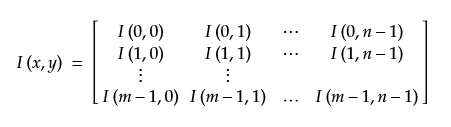
\includegraphics[width=0.8\textwidth]{gambar/image_intensity}
	\caption{Representasi Citra Digital}
	\label{Gambar:imageintensity}
\end{figure}
$m$ x $n$ menyatakan resolusi citra, dan setiap elemen dari matriks menyatakan sebuah piksel (\emph{picture element}). Nilai $I$ pada pasangan koordinat $(x,y)$ disebut intensitas (\emph{intensity}). Dalam operasi pengolahan citra, sebagian besar operasi dilakukan dalam citra \emph{grayscale} \citep{tyagi2018understanding}.

\subsection{Citra \emph{Grayscale}}
Citra \emph{grayscale} adalah citra yang hanya memiliki satu kanal (\emph{channel}) pada setiap pikselnya yang mewakili intensitas. Intensitas piksel berada dalam kisaran [0, 255] yang mana hal ini menunjukkan tingkat terangnya atau tingkat cahaya dari suatu pixel. Warna pada citra \emph{grayscale} merupakan warna abu dengan tingkatan dari hitam hingga sampai putih (tingkat keabuan). Kisaran intensitas piksel bernilai 0 artinya hitam dan 255 adalah putih (untuk \emph{256-graylevel}).
\begin{figure}[H]
	\centering
	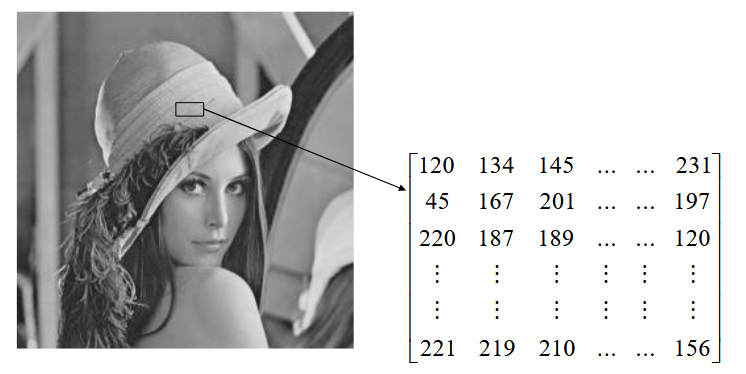
\includegraphics[width=0.5\textwidth]{gambar/grayimage}
	\caption{Contoh citra \emph{grayscale}}
	\label{Gambar:grayimage}
\end{figure}

Setiap piksel dalam citra umumnya dijelaksan oleh kombinasi tiga nilai intensitas R (\emph{red}), G (\emph{green}),dan B (\emph{blue}). Salah satu cara memetakan nilai tersebut ke satu nilai \emph{grayscale} adalah dengan menggunakan metode \emph{luminosity} \citep{kumar2016gray}.
\begin{equation}
	\label{luminosity}
	L(x,y) = 0.21 R (x,y) + 0.72 G (x,y) + 0.07 B (x,y).
\end{equation}
$L(x,y)$ melambangkan nilai intensitas \emph{grayscale} pada pasangan koordinat $(x, y)$. R, G, dan B masing-masing adalah nilai intensites citra \emph{channel} R (\emph{red}), G (\emph{green}),dan B (\emph{blue}) pada pasangan koordinat $(x,y)$

\begin{figure}[H]
	\centering
	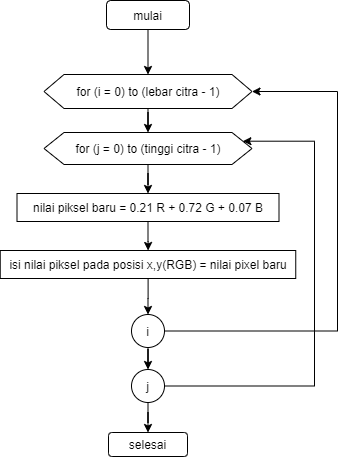
\includegraphics[width=0.45\textwidth]{diagram/grayscale}
	\caption{Proses konversi citra RGB menjadi \emph{grayscale}}
	\label{Gambar:grayscalediagram}
\end{figure}

\subsection{\emph{Gaussian Low Pass Filter} / \emph{Gaussian Filter}}
Peningkatan kualitas citra (\emph{image enhancement}) adalah proses mengedit citra untuk membuatnya 'lebih baik' untuk aplikasi tertentu \citep{tyagi2018understanding}. Hal ini melibatkan proses menghaluskan atau mempertajam konten citra. Salah satu metode dalam proses menghaluskan citra adalah \emph{filtering}, salah satunya adalah dengan menggunakan metode \emph{Gaussian filter}. Proses ini adalah proses memblur citra menggunakan fungsi Gaussian dengan tujuan mengurangi \emph{noise} citra dan mengurangi detail tertentu. Kernel gaussian \emph{Gaussian blur} $G(x,y)$ dideskripsikan sebagai berikut:
\begin{equation}
\label{gaussblur}
G(x,y) = {\frac{1}{2 \pi \sigma^2} e}^{-{\frac{x^2+y^2}{2 \sigma^2}}}
\end{equation}
$\sigma$ dan $e$ menujukkan standar deviasi dan konstanta logaritma natural ($e \approx 2,718281828459$), $x$ dan $y$ adalah posisi koordinat Kernel gaussian.



\section{Gradien citra (\emph{image gradient})}
Tepi (\emph{edge}) dalam ruang lingkup pengolahan citra digital mencirikan batas dari suatu objek dalam citra digital. Deteksi tepi (\emph{edge detection}) merupakan metode identifikasi objek dalam citra berbasis tepi. Salah satu metode deteksi tepi yang umum digunakan adalah metode gradien citra (\emph{image gradient}). Dalam konsep matematis, gradien dikenal sebagai turunan pertama (\emph{first-order derivatives}). Gradien dari citra $I$ dilambangkan dengan notasi $\nabla I$ dan di definisikan sebagai berikut:
\begin{equation}
	\label{gradientimagedefinition}
	{
		\nabla I =
	}
	{
		\begin{bmatrix}
			\nabla I (x,y)_x	\\
			\nabla I (x,y)_y
		\end{bmatrix}
	}
	{
		=
	}
	{
		\begin{bmatrix}
			\frac{\partial I (x,y)}{\partial x}	\\
			\frac{\partial I (x,y)}{\partial y}
		\end{bmatrix}
	}
\end{equation}
di mana $\nabla I (x,y)_x$ dan $\nabla I (x,y)_y$ masing-masing adalah persamaan gradien citra $I$ arah (\emph{direction}) $x$ dan $y$ yang dapat dihitung menggunakan dua persamaan berikut:
\begin{equation}
	\label{gradient_fd1}
	\nabla I (x,y)_x = I(x+1 , y) - I(x,y)
\end{equation}
\begin{equation}
	\label{gradient_fd2}
	\nabla I (x,y)_y = I(x , y + 1) - I(x,y)
\end{equation}
untuk besarnya (\emph{magnitude}) gradien $I$ dapat dihitung menggunakan persamaan berikut:
\begin{equation}
	\label{magnitudegradientfd}
	M(x,y) = ||\nabla I(x,y)|| = \sqrt{ (\nabla I (x,y)_x)^2 + (\nabla I (x,y)_y)^2 }
\end{equation}

Selain menggunakan persamaan (\ref{gradient_fd1}), (\ref{gradient_fd2}), dan (\ref{magnitudegradientfd}), perhitungan gradien citra dapat menggunakan operator gradien yang nantinya akan dikonvolusikan dengan citra. Salah satu operator gradien umum yang sering digunakan adalah operator Sobel/kernel Sobel. Konvolusi dilambangkan dengan $\ast$. Operator Sobel arah $x$ dan $y$, serta besar gradien Sobel masing-masing ditunjukkan oleh persamaan berikut:
\begin{equation}
	\label{sobel_x}
	G_x = 
	\begin{bmatrix}
		-1 & 0 & 1	\\
		-2 & 0 & 2	\\
		-1 & 0 & 1	
	\end{bmatrix}
\end{equation}
\begin{equation}
	\label{sobel_y}
	G_y = 
	\begin{bmatrix}
		1 & 2 & 1	\\
		0 & 0 & 0	\\
		-1 & -2 & -1	
	\end{bmatrix}
\end{equation}
\begin{equation}
	\label{sobel_mag}
	GS = | G_x \ast I(x,y) | + | G_y \ast I(x,y) |
\end{equation}

\begin{figure}[H]
	\centering
	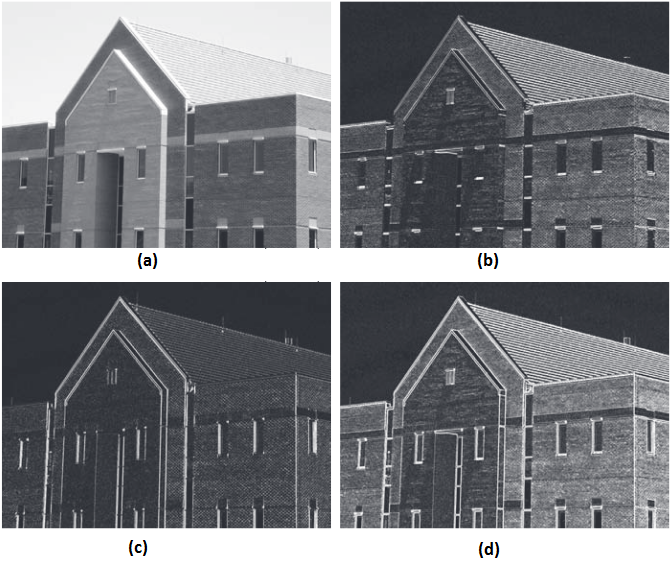
\includegraphics[width=0.8\textwidth]{gambar/sobel}
	\caption{(a) citra \emph{grayscale} ; (b) $|G_x \ast I(x,y)|$, gradien arah $x$ menggunakan kernel Sobel-x ; (c) $|G_y \ast I(x,y)|$, gradien arah $x$ menggunakan kernel Sobel-y ; (d) gradien citra, $| G_x \ast I(x,y) | + | G_y \ast I(x,y) |$ \citep{gonzalez2002digital}}
	\label{Gambar:sobel}
\end{figure}

\section{\emph{Active contour}}
\emph{Active contour} yang juga dikenal dengan sebutan \emph{snakes} adalah kurva yang di definisikan dalam citra (\emph{image}), kurva ini dapat bergerak menuju batas objek atau \emph{feature} dari sebuah citra yang dipengaruhi oleh dua fungsional energi yang disebut energi internal dan energi eksternal.
\begin{figure}[H]
	\centering
	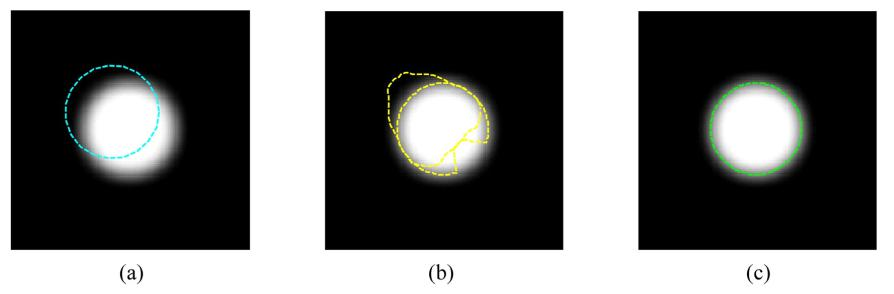
\includegraphics[width=1\textwidth]{gambar/snake1}
	\caption{(a) citra objek lingkaran \& \emph{initial snake}, (b) evolusi kurva \emph{snake},
		(c) bentuk akhir dari \emph{snake} setelah iterasi selesai \citep{acton2007biomedical:19}}
	\label{Gambar:snake1}
\end{figure}

\subsection{Representasi \emph{Snake}}
\emph{Snake} di representasikan sebagai kurva parametrik tertutup $\textbf{v}(s) = (x(s), y(s))$, di mana $s$ adalah panjang kurva dengan rentang tertentu, $x(s)$ dan $y(s)$ masing-masing merupakan elemen dari kurva $\textbf{v}$ pada saat $s$. Sebagai contoh diberikan sebuah kurva sebagai berikut:
\begin{figure}[H]
	\centering
	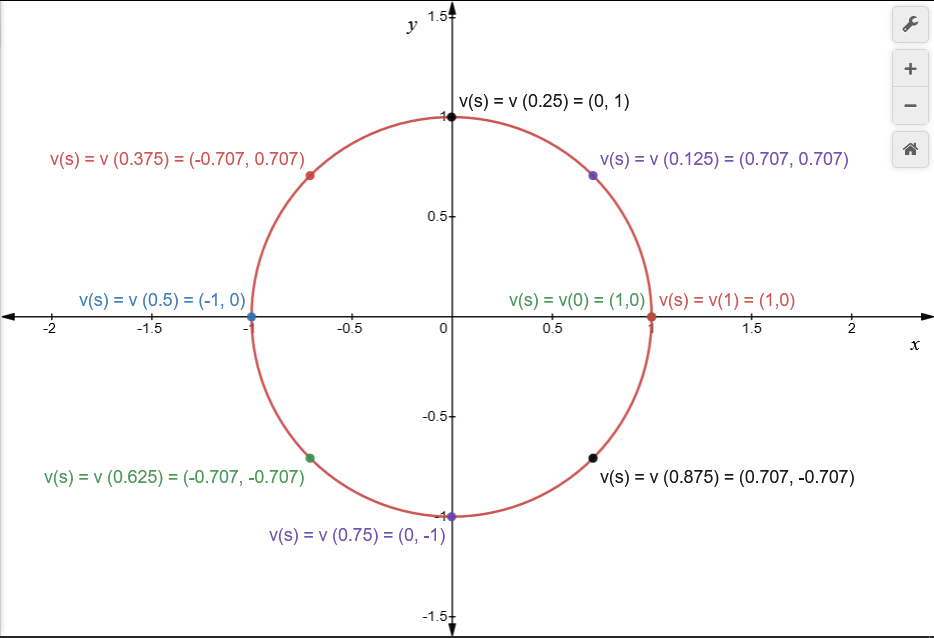
\includegraphics[width=1\textwidth]{gambar/k_lingkaran}
	\caption{Kurva ingkaran}
	\label{Gambar:k_lingkaran}
\end{figure}
Kurva di atas adalah kurva lingkaran $\textbf{v}(s) = [cos (2 \pi s), sin (2 \pi s)]$, $s \in [0, 1]$. Perlu diperhatikan bahwa titik awal $\textbf{v}(0)$ dan titik akhir $\textbf{v}(1)$ di definisikan sebagai titik yang sama.

Algoritma pembuatan lingkaran menggunakan bentuk parametrik (\emph{parametric form}) lingkaran adalah sebagai berikut:
\begin{figure}[H]
	\begin{lstlisting}[language=Python, basicstyle=\tiny]
		repeat until theta >= 360;
		{ 
			x = h + r*cos(theta)
			y = k + r*sin(theta)
			draw a line to x,y
			add step to theta
		}
	\end{lstlisting}
	\caption{\emph{source code} inisialisasi kurva lingkaran}
	\label{Gambar:algo_circle}
\end{figure}
yang dilakukan algoritma di atas adalah menghasilkan koordinat \texttt{x, y} dari sebuah titik pada lingkaran yang diberi sudut (\texttt{theta}). Dimulai dari \texttt{theta = 0} kemudian \emph{looping} sampai \texttt{theta = 360} atau \texttt{theta = $2\pi$}. \texttt{h} dan \texttt{k} adalah koordinat dari titik tengah lingkaran dan \texttt{r} adalah jari-jari lingkaran \citep{john_page}

Fungsional energi \emph{snake} di definisikan sebagai berikut \citep{abdullah2016robust}:
\begin{equation}
	\label{eq_1}
	E_{snake} = \int^1_0 E_{int}(\textbf{v}(s)) ds + \int^1_0 E_{ext}(\textbf{v}(s)) ds.
\end{equation}

\subsection{Energi internal}
Energi internal digunakan untuk mengontrol perubahan bentuk (deformabilitas) dari \emph{snake}, yang ditulis sebagai berikut \citep{abdullah2016robust}:
\begin{equation}
	\label{eq_2}
	E_{int}(\textbf{v}(s)) = \frac{1}{2}  \biggl( \alpha(s)|\textbf{v}_{s}(s)|^2 + \beta(s)|\textbf{v}_{ss}(s)|^2 \biggr)
\end{equation}
$s$ pada $\textbf{v}_{s}$ melambangkan turunan pertama, $ss$ pada $\textbf{v}_{ss}$ melambangkan turunan kedua, dan seterusnya. Fungsi energi internal ini terdiri dari suku pertama yang dikendalikan oleh $\alpha(s)$ dan suku kedua yang dikendalikan oleh $\beta(s)$. Suku pertama mengontrol elastisitas (\emph{elasticity}) dan suku kedua mengontrol kekakuan (\emph{stiffness}) snake. Untuk penyederhanaan, bobot $\alpha(s)$ dan $\beta(s)$ \textbf{diasumsikan seragam}, sehingga $\alpha(s) = \alpha$ dan $\beta(s) = \beta$ hal ini mencegah agar deformabilitas snake tidak membentuk sudut \citep{ivins1995everything}. Tidak ada aturan dalam menentukan $\alpha$ dan $\beta$, tetapi yang perlu diperhatikan adalah semakin kecil nilai $\alpha$ mengakibatkan jarak tiap titik pada kurva semakin tidak teratur dan sebaliknya semakin besar nilai $\alpha$ mengakibatkan jarak tiap titik pada kurva semakin teratur. Untuk parameter $\beta$, semakin kecil nilainya akan menyebabkan bentuk kurva menjadi semakin tidak \emph{smooth} atau dapat membentuk sudut dan sebaliknya semakin besar nilai $\beta$ menyebabkan kurva semakin \emph{smooth} \citep{ickhsan2020implementasi}.

\subsection{Energi eksternal}
Energi internal berasal dari kurva \emph{snake}, sedangkan energi eksternal berasal dari luar yakni dari citra itu sendiri.

Jika diberikan citra tingkat abu-abu (\emph{gray-level image}) $I (x, y)$, maka fungsi energi eksternal yang sesuai meliputi \citep{xu1998snakes:22}:
\begin{equation}
	\label{eext1}
	E^{(1)}_{ext}(x,y) = -|\nabla I(x,y)|^2
\end{equation}
\begin{equation}
	\label{eext2}
	E^{(2)}_{ext}(x,y) =  -|\nabla \left[ G_{\sigma} (x,y) * I(x,y) \right]|^2
\end{equation}
Jika citra tersebut adalah citra biner (\emph{black-white}), energi eksternal yang sesuai di antaranya adalah sebagai berikut:
\begin{equation}
	\label{eext3}
	E^{(3)}_{ext}(x,y) = I(x,y)
\end{equation}
\begin{equation}
	\label{eext4}
	E^{(4)}_{ext}(x,y) = G_{\sigma} (x,y) * I(x,y)
\end{equation}
di mana $G_{\sigma}(x,y)$ adalah fungsi \emph{Gaussian} dengan standar deviasi $\sigma$, $\nabla$ adalah operator gradien. $\ast$ mewakili konvolusi $G_{\sigma}(x,y) \ast I(x,y)$, di mana $I(x,y)$ adalah fungsi intensitas citra. $\nabla$ adalah operator gradien, kita dapat menggunakan operator Sobel pada persamaan (\ref{sobel_x}) dan (\ref{sobel_y}) untuk menjalankan fungsi energi eksternal ini.

Substitusi Energi internal (\ref{eq_2}) dan Energi Eksternal (\ref{eext1}) - (\ref{eext4}) ke fungsional energi \emph{snake} (\ref{eq_1}), menghasilkan persamaan energi \emph{snake} menjadi:
\begin{multline}
\label{eq_4}
E_{snake} = \int^{1}_{0} \Biggl( \frac{1}{2} \biggl(\alpha(s)|\textbf{v}_{s}(s)|^2 + \beta(s)|\textbf{v}_{ss}(s)|^2\biggr) + E^{(i)}_{ext}(x,y) \Biggr) ds.
\end{multline}
dengan $i = 1,2,3,4$.




\section{\emph{Active contour evolution}}
Kurva \emph{snake} akan bergerak menuju batas dari \emph{feature} dari sebuah citra, proses ini disebut \emph{active contour evolution}. Perhitungan evolusi \emph{snake} yang meminimalkan persamaan energi (\ref{eq_4}) ketika $\alpha(s) = \alpha$ dan $\beta(s) = \beta$, harus memenuhi persamaan Euler berikut \citep{xu1998snakes:22}:
\begin{equation}
	\label{snake_euler}
	\alpha\textbf{v}_{ss}(s) - \beta\textbf{v}_{ssss}(s) + \nabla E^{(i)}_{ext}  = 0
\end{equation}
Untuk menemukan solusi persamaan (\ref{snake_euler}), kurva snake $\textbf{v}$ dibuat dinamis terhadap waktu $t$. Turunan parsial $\textbf{v}$ terhadap $t$ ditetapkan sama dengan ruas kiri persamaan (\ref{snake_euler}) sebagai berikut \citep{xu1998snakes:22}:
\begin{equation}
	\label{snake_euler_t}
	\textbf{v}_{t}(s,t) = \alpha\textbf{v}_{ss}(s,t) - \beta\textbf{v}_{ssss}(s,t) + \nabla E^{(i)}_{ext}  = 0
\end{equation}
atau dapat ditulis sebagai berikut \citep{ivins1995everything}:
\begin{equation}
	\label{snake_euler_t_partial}
	\frac{\partial\textbf{v}}{\partial t} = \alpha \frac{\partial^2 \textbf{v}}{\partial s^2} - \beta \frac{\partial^4 \textbf{v}}{\partial s^4} + \frac{\partial E^{(i)}_{ext} }{ \partial \textbf{v}} = 0
\end{equation}
$\textbf{v}$ pada persmaan (\ref{snake_euler_t_partial}) dapat dipisahkan menjadi komponen/elemen $x$ dan $y$, katakanlah $u_{j}$ adalah komponen/elemen \emph{snake} $\textbf{v}$ di mana $j = 0,1,.., N-1$ sebagai aproksimasi diskrit untuk $x(s)$ dan $y(s)$, dan $t$ melambangkan iterasi, maka persamaan (\ref{snake_euler_t_partial}) menjadi:
\begin{equation}
	\label{snake_euler_t_partial_u}
	\frac{\partial u^{t}_{j} }{\partial t} = \alpha \frac{\partial^2 u^{t}_{j}}{\partial s^2} - \beta \frac{\partial^4 u^{t}_{j}}{\partial s^4} + \frac{\partial E^{(i)}_{ext} }{ \partial u^{t}_{j}} = 0
\end{equation}
Turunan pada persamaan (\ref{snake_euler_t_partial_u}) dapat diaproksimasikan menggunakan \emph{finite differences} yang ditunjukan pada gambar berikut:
\begin{figure}[H]
	\centering
	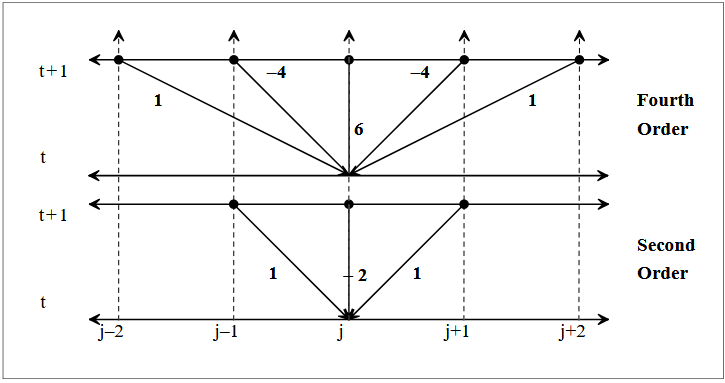
\includegraphics[width=1\textwidth]{gambar/finite_d}
	\caption{Aproksimasi turunan dengan \emph{finite differences} \citep{ivins1995everything}}
	\label{Gambar:finite_d}
\end{figure}
Turunan $\frac{\partial u^{t}_{j} }{\partial t}$ diaproksimasikan menjadi $\dfrac{ u^{t+1}_j - u^{t}_j }{\delta t}$ \citep{ivins1995everything}. Turunan orde kedua, yaitu $\frac{\partial^2 u^{t}_{j}}{\partial s^2}$ diaproksimasikan menjadi $\frac{( u^{t+1}_{j+1} + u^{t+1}_{j-1} - 2u^{t+1}_{j} )}{\delta s^2}$, sedangkan turunan orde keempat, yaitu $\frac{\partial^4 u^{t}_{j}}{\partial s^4}$ diaproksimasikan menjadi $\frac{( u^{t+1}_{j+2} - 4u^{t+1}_{j+1} + 6u^{t+1}_{j} - 4u^{t+1}_{j-1} + u^{t+1}_{j-2})}{\delta s^4}$.
Turunan dalam persamaan (\ref{snake_euler_t_partial_u}) yang diaproksimasi menggunakan \emph{finite differences} seperti yang ditunjukkan pada Gambar (\ref{Gambar:finite_d}) adalah sebagai berikut:

\begin{multline}
	\label{aprox_finite}
	\dfrac{ u^{t+1}_j - u^{t}_j }{\delta t} = \frac{\alpha}{\delta s^2}( u^{t+1}_{j+1} + u^{t+1}_{j-1} - 2u^{t+1}_{j} ) \\
	- \frac{\beta}{\delta s^4}( u^{t+1}_{j+2} - 4u^{t+1}_{j+1} + 6u^{t+1}_{j} - 4u^{t+1}_{j-1} + u^{t+1}_{j-2}) + \frac{\partial E^{(i)}_{ext} }{ \partial u^{t}_{j}}
\end{multline}

\begin{comment}
\begin{multline}
	\label{aprox_finite1}
	u^{t+1}_j - u^{t}_j = \frac{\alpha \delta t}{\delta s^2} u^{t+1}_{j+1} + \frac{\alpha \delta t}{\delta s^2} u^{t+1}_{j-1} - \frac{\alpha \delta t}{\delta s^2} 2u^{t+1}_{j} \\
	- \frac{\beta \delta t}{\delta s^4} u^{t+1}_{j+2} + \frac{\beta \delta t}{\delta s^4} 4u^{t+1}_{j+1} - \frac{\beta \delta t}{\delta s^4} 6u^{t+1}_{j} + \frac{\beta \delta t}{\delta s^4} 4u^{t+1}_{j-1} - \frac{\beta \delta t}{\delta s^4} u^{t+1}_{j-2} - \frac{\partial E^{(i)}_{ext} \delta t}{ \partial u^{t}_{j}}
\end{multline}

\begin{multline}
	\label{aprox_finite2}
	u^{t+1}_j - u^{t}_j = \frac{\alpha \delta t}{\delta s^2} u^{t+1}_{j+1} + \frac{\alpha \delta t}{\delta s^2} u^{t+1}_{j-1} - \frac{\alpha \delta t}{\delta s^2} 2u^{t+1}_{j} \\
	- \frac{\beta \delta t}{\delta s^4} u^{t+1}_{j+2} + \frac{\beta \delta t}{\delta s^4} 4u^{t+1}_{j+1} - \frac{\beta \delta t}{\delta s^4} 6u^{t+1}_{j} + \frac{\beta \delta t}{\delta s^4} 4u^{t+1}_{j-1} - \frac{\beta \delta t}{\delta s^4} u^{t+1}_{j-2} - \frac{\partial E^{(i)}_{ext} \delta t}{ \partial u^{t}_{j}}
\end{multline}
\end{comment}


di mana $t$ dan $t+1$ mewakili parameter waktu yang berurutan dengan langkah waktu (\emph{time step}) $\delta t$. $\delta s$ mewakili ukuran langkah (\emph{step size}). Mememindahkan $\delta t$ ke ruas kanan persamaan membuat persamaan (\ref{aprox_finite}) menjadi:
\begin{multline}
	\label{aprox_finite_LHS}
	b u^{t+1}_{j+2} - (a+4b) u^{t+1}_{j+1} + (1+2a+6b) u^{t+1}_{j} - (a+4b) u^{t+1}_{j-1} + b u^{t+1}_{j-2} \\
	= u^{t}_{j} + \delta t \frac{\partial E^{(i)}_{ext} }{ \partial u^{t}_{j}}
\end{multline}
di mana $a \equiv \alpha \frac{\delta t}{\delta s^2} $ dan $b \equiv \beta \frac{\delta t}{\delta s^4} $.
Persamaan (\ref{aprox_finite_LHS}) dapat juga ditulis sebagai berikut:
\begin{equation}
	\label{aprox_finite_rhs}
	p u^{t+1}_{j+2} + q u^{t+1}_{j+1} + r u^{t+1}_{j} + q u^{t+1}_{j-1} + p u^{t+1}_{j-2} \\
	= \tilde{u}^{t+1}_{j}
\end{equation}
di mana $p \equiv b$, $q \equiv -a-4b$, dan $r \equiv 1+2a+6b$, sedangkan $\tilde{u}^{t+1}_{j} = u^{t}_{j} + \delta t \frac{\partial E^{(i)}_{ext} }{ \partial u^{t}_{j}}$. Persamaan (\ref{aprox_finite_rhs}) ini dapat ditulis dalam bentuk matriks untuk koordinat $x$ dan $y$ dari setiap elemen kurva \emph{snake} $\textbf{v}$.



\begin{equation}
	\label{matriks_implicit}
	{
		\begin{bmatrix}
			r 	& q			& p 	 & 		  & 	   & p 		& q \\
			q 	& r     	& q 	 & 	p	  & 	   &  		& p \\
			p 	& q     	& r 	 & 	q	  & p	   &  		&  	\\
			& \ddots 	& \ddots & \ddots & \ddots & \ddots &  	\\
			&  			& p 	 & 	q	  & r	   & q 		& p \\
			p 	&  			& 	 	 & 	p	  & q	   & r 		& q \\
			q 	& p 		&  		 & 		  & p	   & q 		& r
		\end{bmatrix}
	}
	{
		\begin{bmatrix}
			u^{t+1}_{0} 	\\
			u^{t+1}_{1} 	\\
			u^{t+1}_{2} 	\\
			\vdots 			\\
			u^{t+1}_{N-3}\\
			u^{t+1}_{N-2}\\
			u^{t+1}_{N-1}
		\end{bmatrix}
	}
	{
		=
	}
	{
		\begin{bmatrix}
			\tilde{u}^{t+1}_{0} 	\\
			\tilde{u}^{t+1}_{1} 	\\
			\tilde{u}^{t+1}_{2} 	\\
			\vdots 					\\
			\tilde{u}^{t+1}_{N-3}	\\
			\tilde{u}^{t+1}_{N-2}	\\
			\tilde{u}^{t+1}_{N-1}
		\end{bmatrix}
	}
\end{equation}
di mana

\begin{equation}
	\label{matriks_m}
	{
		\textbf{M} =
	}
	{
		\begin{bmatrix}
			r 	& q			& p 	 & 		  & 	   & p 		& q \\
			q 	& r     	& q 	 & 	p	  & 	   &  		& p \\
			p 	& q     	& r 	 & 	q	  & p	   &  		&  	\\
			& \ddots 	& \ddots & \ddots & \ddots & \ddots &  	\\
			&  			& p 	 & 	q	  & r	   & q 		& p \\
			p 	&  			& 	 	 & 	p	  & q	   & r 		& q \\
			q 	& p 		&  		 & 		  & p	   & q 		& r
		\end{bmatrix}
	}
\end{equation}

\begin{equation}
	\label{matriks_ut1}
	{
		\textbf{u}^{t+1}_{j} =
	}
	{
		\begin{bmatrix}
			u^{t+1}_{0} 	\\
			u^{t+1}_{1} 	\\
			u^{t+1}_{2} 	\\
			\vdots 			\\
			u^{t+1}_{N-3}\\
			u^{t+1}_{N-2}\\
			u^{t+1}_{N-1}
		\end{bmatrix}
	}
\end{equation}

\begin{equation}
	\label{matriks_ut2}
	{
		\tilde{\textbf{u}}_{j}^{t+1} =
	}
	{
		\begin{bmatrix}
			\tilde{u}^{t+1}_{0} 	\\
			\tilde{u}^{t+1}_{1} 	\\
			\tilde{u}^{t+1}_{2} 	\\
			\vdots 					\\
			\tilde{u}^{t+1}_{N-3}	\\
			\tilde{u}^{t+1}_{N-2}	\\
			\tilde{u}^{t+1}_{N-1}
		\end{bmatrix}
	}
	{
		=
	}
	{
		\begin{bmatrix}
			u^{t}_{0} + \delta t \frac{\partial E^{(i)}_{ext} }{ \partial u^{t}_{0}} 	\\
			u^{t}_{1} + \delta t \frac{\partial E^{(i)}_{ext} }{ \partial u^{t}_{1}} 	\\
			u^{t}_{2} + \delta t \frac{\partial E^{(i)}_{ext} }{ \partial u^{t}_{2}} 	\\
			\vdots 					\\
			u^{t}_{N-3} + \delta t \frac{\partial E^{(i)}_{ext} }{ \partial u^{t}_{N-3}}	\\
			u^{t}_{N-2} + \delta t \frac{\partial E^{(i)}_{ext} }{ \partial u^{t}_{N-2}}	\\
			u^{t}_{N-1} + \delta t \frac{\partial E^{(i)}_{ext} }{ \partial u^{t}_{N-1}}
		\end{bmatrix}
	}
	%{
	%	=
	%}
	%{
	%	u^{t}_{j} - \delta t \frac{\partial E^{(i)}_{ext} }{ \partial u^{t}_{j}}
	%}
\end{equation}

\begin{equation}
	\label{consteq}
	p \equiv \beta \frac{\delta t}{\delta s^4}, q \equiv - \alpha \frac{\delta t}{\delta s^2} - 4 \beta \frac{\delta t}{\delta s^4}, r \equiv  1 + 2 \alpha \frac{\delta t}{\delta s^2} + 6 \beta \frac{\delta t}{\delta s^4}
\end{equation}
Mengalikan kedua sisi dari persamaan (\ref{matriks_implicit}) dengan inverse dari matriks $\textbf{M}$ memberikan solusi akhir persamaan \emph{snake} menjadi:
\begin{equation}
	\label{implicit}
	\textbf{u}^{t+1}_{j} = \textbf{M}^{-1} \biggl( \textbf{u}^t_{j} + \delta t  \frac{\partial E^{(i)}_{ext} }{ \partial \textbf{u}^{t}_{j}} \biggr)
\end{equation}

Perlu diingat $\textbf{u}$ adalah komponen/elemen $x$ dan $y$ pada kurva \emph{snake}, komponen/elemen ini dapat dinyatakan dengan vektor $\textbf{x}$ dan $\textbf{y}$. Jika $E^{(i)}_{ext}$ dinotasikan menjadi fungsi $\textbf{f}$ maka :
\begin{equation}
	\label{ext_f}
	\frac{\partial E^{(i)}_{ext} }{ \partial \textbf{u}^{t}_{j}} = \frac{\partial \textbf{f} }{ \partial \textbf{u}^{t}_{j}}
\end{equation}

Hal ini membuat persamaan (\ref{implicit}) dapat ditulis sebagai berikut:
\begin{equation}
	\label{implicit_x}
	\textbf{x}^{t+1}_{j} = \textbf{M}^{-1} \biggl( \textbf{x}^t_{j} + \delta t \; \textbf{f}_{x} \biggr)
\end{equation}
dan
\begin{equation}
	\label{implicit_y}
	\textbf{y}^{t+1}_{j} = \textbf{M}^{-1} \biggl( \textbf{y}^t_{j} + \delta t \; \textbf{f}_{y} \biggr)
\end{equation}

$\textbf{f}_x$ dan $\textbf{f}_y$ adalah vektor-vektor yang bersesuaian dengan bentuk turunan pertama $\frac{\partial \textbf{f} }{ \partial \textbf{u}^{t}_{j}}$ sebagai berikut:
\begin{equation}
	\label{fx_eq}
	% \textbf{f}_x = f_x(x^t_{j}, y^t_{j}) = f(x^t_{j}+1) , y^t_{j}) - f(x^t_{j},y^t_{j})
	\textbf{f}_x = f_x(x^t_{j}, y^t_{j})
\end{equation}

\begin{equation}
	\label{fy_eq}
	% \textbf{f}_y = f_y(x^t_{j}, y^t_{j}) = f(x^t_{j}, y^t_{j}+1) - f(x^t_{j},y^t_{j})
	\textbf{f}_y = f_y(x^t_{j}, y^t_{j})
\end{equation}
di mana $x^t_{j}$ dan $y^t_{j}$ adalah pasangan koordinat dari kurva \emph{snake}. $\textbf{f}_x$ dan $\textbf{f}_y$ dapat dicari menggunakan teori gradien citra.
%--algoritma ,equilibrium--

\section{Interpolasi Bilinear}
Interpolasi Bilinear adalah metode interpolasi fungsi dari dua variabel (misal $x$ dan $y$). Metode ini biasanya digunakan untuk mengaproksimasi nilai data di antara beberapa titik dalam \emph{2D rectangular grid}, misalnya di dalam matriks \citep{william1997numerical}.

Misal kita ingin mencari nilai fungsi $f$ yang tidak diketahui di titik $(x,y)$ dan diasumsikan kita mengetahui nilai $f$ pada beberapa empat titik $Q_11 = (x_1, y_1), Q_12 = (x_1, y_2), Q_21 = (x_2, y_1), dan Q_22 = (x_2, y_2)$ maka langkah yang harus dilakukan sebagai berikut:
\begin{equation}
	\label{bilin_x1}
	f(x,y_1) = \frac{x_2 - x}{x_2 - x1} f(Q_11) + \frac{x - x_1}{x_2 - x_1} f(Q_21) = R1
\end{equation}

\begin{equation}
	\label{bilin_x2}
	f(x,y_2) = \frac{x_2 - x}{x_2 - x1} f(Q_12) + \frac{x - x_1}{x_2 - x_1} f(Q_22) = R2
\end{equation}

\begin{equation}
	\label{bilin_y}
	f(x,y) = \frac{y_2 - y}{y_2 - y_1} f(x, y_1) + \frac{y - y_1}{y_2 - y_1} f(x, y_2) = P
\end{equation}

\begin{figure}[H]
	\centering
	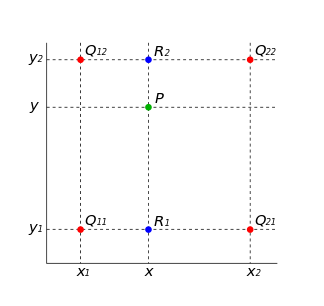
\includegraphics[width=.7\textwidth]{gambar/bilinear_interpolation}
	\caption{interpolasi bilinear}
	\label{Gambar:bilin_ilust}
\end{figure}


\begin{comment}

\section{\emph{Gradient Vector Flow (GVF) snake}}
Model \emph{snake} tradisional memiliki kekurangan seperti yang dibahas sebelumnya. Sebagian besar alasan kinerja yang buruk dikaitkan dengan energi eksternal. Untuk memperbaiki masalah ini, \citep{xu1998snakes:22} mengusulkan energi eksternal baru yang dikenal sebagai GVF \emph{snake} . 

Model dasar GVF sama dengan persamaan \emph{snake} (\ref{snake_euler_t}), tetapi yang membedakan adalah energi eksternal $- \nabla E^{(i)}_{ext}$ yang di definisikan menjadi $\textbf{g}$ sebagai berikut:
\begin{equation}
	\label{gvf_euler_t}
	\textbf{v}_{t}(s,t) = \alpha\textbf{v}_{ss}(s,t) - \beta\textbf{v}_{ssss}(s,t) + \textbf{g}  = 0
\end{equation}
di mana $\textbf{g}(x, y) = [ u (x, y), v (x, y) ]$ adalah bidang vektor(\emph{vector field}), \emph{field} ini dapat dianggap sebagai \textbf{vektor gradien} dari citra (\emph{gray-level} atau \emph{binary edge-map}) \citep{xu1998snakes:22}.

\subsection{Peta Tepi (\emph{Edge Map})}
Langkah pertama untuk mendapatkan GVF adalah mendefinisikan fungsi \emph{edge map} $f(x,y)$ yang berasal dari citra $I(x,y)$. Kita dapat menggunakan peta tepi \emph{gray-level} atau \emph{binary} sesuai yang kita tentukan berdasarkan energi eksternal \emph{snake} dasar pada persamaan (\ref{eext1}) - (\ref{eext4}) sebagai berikut:
\begin{equation}
	\label{gvf_edge_map}
	f(x,y) = - E^{(i)}_{ext}(x,y)
\end{equation}
dengan $i = 1,2,3,4$.


%================|||||=====================



\subsection{\emph{Gradient Vector Flow}}
\emph{GVF} di definisikan sebagai vektor gradien $\textbf{g}(x,y) = [u(x,y), v(x,y)]$ yang meminimalkan fungsional energi sebagai berikut
\begin{equation}
	\label{equ_gvf}
	\varepsilon = \int \int \mu (u_x^2 + u_y^2 + v_x^2 + v_y^2) + |\nabla f|^2 |\textbf{g} - \nabla f|^2 \,\, dx dx
\end{equation}
di mana $\nabla f$ adalah gradien dari \emph{edge map}. $\mu$ adalah parameter regularisasi (\emph{regularization parameter}) yang menyesuaikan antara suku pertama dan suku kedua. Parameter $\mu$ dikenal sebagai pemulusan (\emph{smoothing term}) dan data(\emph{data term}). Nilai $\mu$ bergantung pada tingkat kebisingan(\emph{noise}) yang ada pada citra $I$, yaitu semakin tinggi \emph{noise}, nilai $\mu$ sebaiknya ditingkatkan\citep{xu1998snakes:22}.

Persamaan (\ref{equ_gvf}) bukan merupakan bentuk akhir karena masih dalam bentuk integran. Untuk mencari nilai $\textbf{g}$, dua persamaan Euler dibawah ini harus diselesaikan:
\begin{equation}
	\label{equ_gvf_a1}
	\mu {\nabla}^2 u - (u - f_x) (f_x^2 + f_y^2) = 0
\end{equation}
dan
\begin{equation}
	\label{equ_gvf_a2}
	\mu {\nabla}^2 v - (v - f_y) (f_x^2 + f_y^2) = 0
\end{equation}
dengan ${\nabla}^2$ adalah operator Laplacian. Untuk menghitung $f_x$ dan $f_y$ dapat menggunakan operator gradien umum seperti operator Sobel pada persamaan (\ref{sobel_x}) dan (\ref{sobel_y}). Kedua persamaan di atas dapat diselesaikan dengan menjadikan $u$ dan $v$ sebagai fungsi waktu $t$ sebagai berikut:
\begin{equation}
	\label{equ_gvf_b1}
	u_t(x,y,t) = \mu {\nabla}^2 u(x,y,t) - [ u(x,y,t) - f_x(x,y) ] [ f^2_x (x,y) + f_y^2(x,y) ]
\end{equation}
dan
\begin{equation}
	\label{equ_gvf_b2}
	v_t(x,y,t) = \mu {\nabla}^2 v(x,y,t) - [ v(x,y,t) - f_y(x,y) ] [ f^2_x (x,y) + f_y^2(x,y) ]
\end{equation}
Persamaan (\ref{equ_gvf_b1}) dan (\ref{equ_gvf_b2}) dapat ditulis ulang sebagai berikut :
\begin{equation}
	\label{gvf_t1}
	u_t(x,y,t) = \mu {\nabla}^2 u(x,y,t) - b(x,y) u(x,y,t) + c^1(x,y)
\end{equation}
dan
\begin{equation}
	\label{gvf_t2}
	v_t(x,y,t) = \mu {\nabla}^2 v(x,y,t) - b(x,y) u(x,y,t) + c^2(x,y)
\end{equation}
di mana
\begin{equation}
	\label{gvf_b}
	b (x,y) = f_x(x,y)^2 + f_y(x,y)^2
\end{equation}
\begin{equation}
	\label{gvf_c1}
	c^1 (x,y) = b(x,y) f_x(x,y)
\end{equation}
\begin{equation}
	\label{gvf_c2}
	c^2 (x,y) = b(x,y)f_y(x,y)
\end{equation}
Untuk solusi iteratif, atur jarak antar piksel menjadi $\Delta x$ dan $\Delta y$, dan langkah waktu(\emph{time step}) untuk setiap iterasi adalah $\Delta t$. Maka selanjutnya dapat diaproksimasikan sebagai berikut\citep{xu1998snakes:22}:
\begin{equation}
	\label{gvf_ut}
	u_t = \frac{1}{\Delta t} ( u^{t+1}_{x,y} - u^t_{x,y} )
\end{equation}
\begin{equation}
	\label{gvf_vt}
	v_t = \frac{1}{\Delta t} ( v^{t+1}_{x,y} - v^n_{x,y} )
\end{equation}
\begin{equation}
	\label{gvf_laplace_u}
	\nabla^2 u = \frac{1}{\Delta x \Delta y} ( u_{x+1,y} + u_{x,y+1} + u_{x-1,y} + u_{x,y-1} - 4u_{x,y} )
\end{equation}
\begin{equation}
	\label{gvf_laplace_v}
	\nabla^2 v = \frac{1}{\Delta x \Delta y} ( v_{x+1,y} + v_{x,y+1} + v_{x-1,y} + v_{x,y-1} - 4v_{x,y} )
\end{equation}
substitusi notasi di atas ke persamaan (\ref{gvf_t1}) dan (\ref{gvf_t2}) memberikan solusi iteratif sebagai berikut
\begin{equation}
	\label{gvfc1}
	u^{t+1}_{x,y} = (1 - b_{i,j} \Delta t) u^{t}_{x,y} + r ( u^{t}_{x+1 , y} + u^t_{x,y+1} + u^t_{x-1 , y} + u^t_{x, y-1} - 4u^t_{x, y}) + c^1_{x,y} \Delta t
\end{equation}
dan
\begin{equation}
	\label{gvfc2}
	v^{t+1}_{x,y} = (1 - b_{x,y} \Delta t) v^{t}_{x,y} + r ( v^{t}_{x+1 , y} + v^n_{x,y+1} + v^t_{x-1 , y} + v^t_{x, y-1} - 4v^t_{x, y}) + c^2_{x,y} \Delta t
\end{equation}
di mana
\begin{equation}
	\label{gvf_r}
	r = \frac{ \mu \Delta t}{\Delta x \Delta y}
\end{equation}
% Selanjutnya jika $\Delta x$, $\Delta y$ dan $\mu$ konstan, maka nilai $\Delta t$ harus memenuhi \citep{CartasAyala2011GradientVF}:
Selanjutnya jika $\Delta x$, $\Delta y$ dan $\mu$ konstan, maka nilai $\Delta t$ harus memenuhi:
\begin{equation}
	\label{gvfnot5}
	\Delta t \leq \frac{\Delta x \Delta y}{4 \mu}
\end{equation}

Selanjutnya dengan mengganti bentuk energi eksternal \emph{snake} dasar masing-masing dengan $u$ dan $v$, persamaan evolusi \emph{snake} (\ref{implicit_x}) dan (\ref{implicit_y})menjadi:
\begin{equation}
	\label{implicit_gvf_u}
	\textbf{x}^{t+1} = \textbf{M}^{-1} \biggl( \textbf{x}^t + \delta t \; u^{t+1}_{x,y} \biggr)
\end{equation}
dan
\begin{equation}
	\label{implicit_gvf_y}
	\textbf{y}^{t+1} = \textbf{M}^{-1} \biggl( \textbf{y}^t + \delta t \; v^{t+1}_{x,y} \biggr)
\end{equation}


berikut adalah ilustrasi dari GVF \emph{snake}:
\begin{figure}[H]
	\centering
	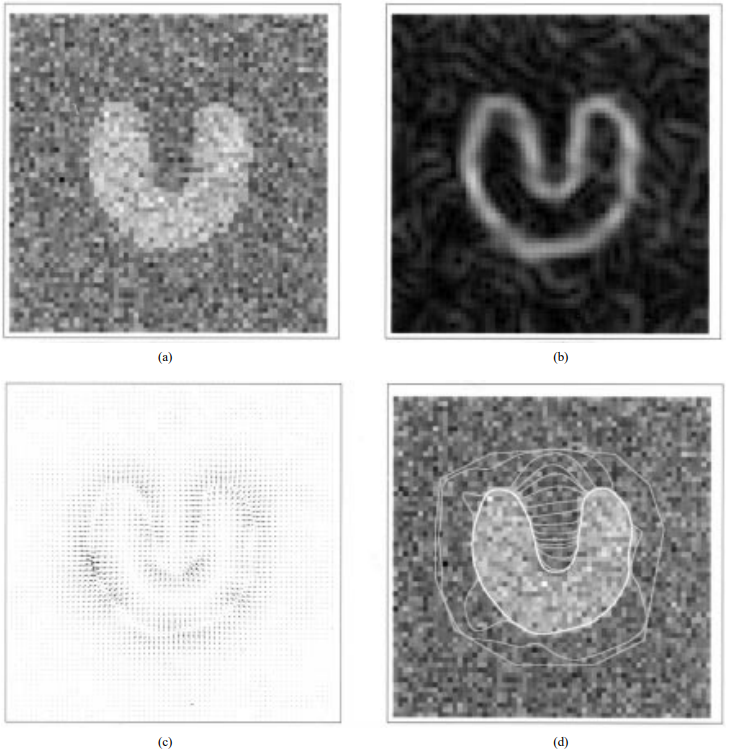
\includegraphics[width=.7\textwidth]{gambar/gvfilu}
	\caption{(a) citra objek U yang memiliki \emph{noise}; (b) \emph{edge map}; (c) medan gaya eksternal GVF; dan (d) konvergensi GVF \emph{snake} \citep{xu1998snakes:22}.}
	\label{Gambar:gvfilu}
\end{figure}

\end{comment}

% Baris ini digunakan untuk membantu dalam melakukan sitasi
% Karena diapit dengan comment, maka baris ini akan diabaikan
% oleh compiler LaTeX.
\begin{comment}
bibliography{daftar-pustaka}
\end{comment}
